\section{Zielsetzung}
\label{sec:Zielsetzung}

Ziel dieses Versuches ist es das Relaxationsverhalten eines RC-Kreises zu untersuchen. 
Dies erfolgt durch Bestimmung der Zeitkonstante, Messung der frequenzabhängigen Amplitude der Kondensatorspannung und 
der frequenzabhängigen Phasenverschiebung zwischen Generator- und Kondensatorspannung.
Außerdem wird gezeigt, dass der RC-Kreis als Integrator arbeiten kann.


\section{Theorie}
\label{sec:Theorie}

\subsection{Allgemeines Relaxationsverfahren} % (fold)
\label{sub:Allgemein}
Relaxation in der Physik ist das nicht-oszillatiorische Zurückkehren in den Ausgangszustand eines Systems, nachdem es daraus entfernt wurde.
Als Beispiel für das Relaxationsphänomen kann die Schaltung in \autoref{fig:Kondensator} benutzt werden. 
\begin{figure}[H]
    \centering
    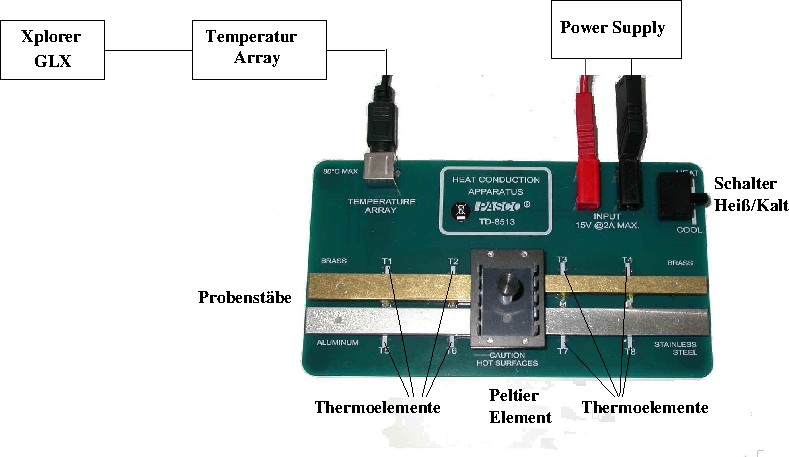
\includegraphics[width=0.5\textwidth]{build/Abb_1.pdf}
    \caption {Auf- und Endladung eines Kondensators über einen Widerstand.\cite{V353}}
    \label{fig:Kondensator}
\end{figure}
\noindent Diese stellt die Auf- und Entladung des Kondensators über einen Widerstand dar.
Die Aufladevorgang beginnt beginnt, wenn der Schalter auf Position $2$ gestellt wird und der Entladevorgang beginnt, wenn der Schalter auf Position $1$ steht.
% subsection Allgemein (end)

\subsection{Entladevorgang eines Kondensators} % (fold)
\label{sub:Entladevorgang}
Der Entladevorgang beginnt, wenn sich auf dem Kondensator die Ladung $Q$ befindet.
Dann liegt zwischen den Platten die Spannung
\begin{equation}
    U_C = \frac{Q}{C}
    \label{eqn:Kondensatorspannung}
\end{equation}
an und nach dem Ohmschen Gesetzt ergibt dies den Strom
\begin{equation}
    I = \frac{U_C}{R} .
\end{equation}
Der zeitliche Verlauf der Ladung lässt sich darstellen durch
\begin{equation}
    Q(t) = Q(0) e^{\frac{-1}{RC}}
    \label{eqn:Ladung_zeitlich}
\end{equation}
,wobei $RC$ eine Zeitkonstante ist, die im nächsten Kapitel näher erläutert wird.
% subsection Entladevorgang (end)


\subsection{Aufladevorgang eines Kondensators} % (fold)
\label{sub:Aufladevorgang}
Beim Aufladevorgang müssen die Randbedingungen
\begin{align}
    Q(0)&=0 &\text{und}&& Q(\infty)=CU_0
\end{align}
gelten. Der Aufladevorgang kann dann durch die Gleichung
\begin{equation}
    Q(t)= CU_0\Bigl(1-e^{\frac{-t}{RC}}\Bigr)
\end{equation}
dargestellt werden. Die Zeitkonstante wird auch hier wieder durch $RC$ ausgedrückt.
Sie ist ein Maß für die Geschwindigkeit, mit der das System seinem Endzustand (hier Q(\infty)) entgegen strebt.
Die Ladung auf dem Kondensator ändert sich um den Faktor
\begin{equation}
    \frac{Q(t)}{Q(0)} = \frac{-t}{RC}
\end{equation}
und für den Zeitraum $\Delta T = RC$ gilt
\begin{equation}
    \frac{Q(t)}{Q(0)} = \frac{1}{e} \approx 0,368 .
\end{equation}


% subsection Aufladevorgang (end)

\subsection{Relaxationsphänomen bei einer periodischen Auslenkung} % (fold)
\label{sub:Rela_peri}
Ein weiteres Relaxationsphänomen ist zum Beispiel bei einer periodischen Auslenkung zu beobachten. Dieses kann auch mit einem RC-Kreis untersucht werden.
\begin{figure}[H]
    \centering
    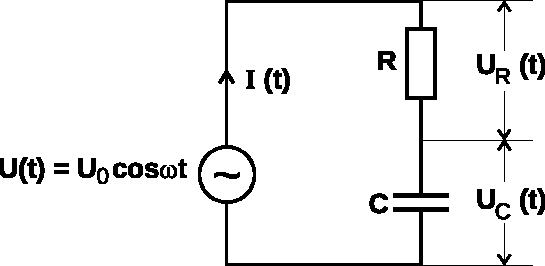
\includegraphics[width=0.5\textwidth]{build/Abb_2.pdf}
    \caption {Beispiel für eine Schaltung zur Diskussion von Relaxationsphänomen unter periodischen Auslenkung.\cite{v353}}
    \label{fig:Abb_2}
\end{figure}
\noindent Es wird eine Schaltung wie in \autoref{fig:Abb_2} aufgebaut und eine Wechselspannung
\begin{equation}
    U(t) = U_0 \text{cos}(\omega t)
    \label{eqn:Wechselspannung}
\end{equation}
mit einer Kreisfrequenz $\omega=2\pi f$ angelegt.
Das Verhalten des RC-Kreises ist abhängig von der Frequenz, so gilt, dass für $\omega << \frac{1}{RC}$ die Kondensatorspannung $U_C$ ungefähr der Wechselspannung $U(t)$ am Generator entspricht.
Bei zunehmender Frequenz kommt es zu einer Phasenverschiebung $\phi$ zwischen den Spannungen, wobei die Generatorspannung der Kondensatorspannung vor läuft.
Dies liegt daran, dass der Auflade- und Entladevorgang zu langsam wird und der Kondensator nicht komplett aufgeladen werden kann. 
Dadurch wird die Amplitude
\begin{equation}
    \frac{A(\omega)}{U_0} = \frac{1}{\sqrt{1+\omega^2R^2C^2}}
    \label{eqn:Amplitude}
\end{equation}
kleiner.\\
\noindent Die Phasenverschiebung nähert sich bei zunehmender Frequenz einem Wert von $\phi =\frac{\pi}{2}$ an und bei niedrigen Frequenzen geht sie gegen $0$.
Sie kann auch beschrieben werden durch
\begin{equation}
    \phi(\omega) = \text{arctan}(-\omega RC).
    \label{eqn:arctan}
\end{equation}
% subsection Relaxationsphänomen bei einer periodischen Auslenkung (end)

\subsection{RC-Kreis als Integrator} % (fold)
\label{sub:Integrator4}
Ein RC-Kreis kann eine zeitlich veränderliche Spannung unter bestimmten Voraussetzungen integrieren.
So gilt, dass wenn die Frequenz $\omega >> \frac{1}{RC}$ beträgt, $U_C$ proportional zu $\int U(t)dt$ ist.
Wenn die Voraussetzungen
\begin{align*}
    \omega&>>\frac{1}{RC},&\lvert U_C\rvert&<< \lvert U_R\rvert &\text{und}&& \lvert U_C\rvert &<< \lvert U\rvert
\end{align*}
gelten, dann kann näherungsweise
\begin{align}
    U(t) &= R\,C \,\frac{dU_C}{dt} &\text{oder} && U_C(t)&= \frac{1}{RC} \int^t_0 U(t') dt'
\end{align}
geschrieben werden.
% subsection  (end)

